\section{Actor-Critic Methods}
\begin{frame}{}
    \LARGE Policy Optimization: \textbf{Actor-Critic Methods}
\end{frame}

\begin{frame}{The Two Worlds of RL}
\begin{figure}
\centering
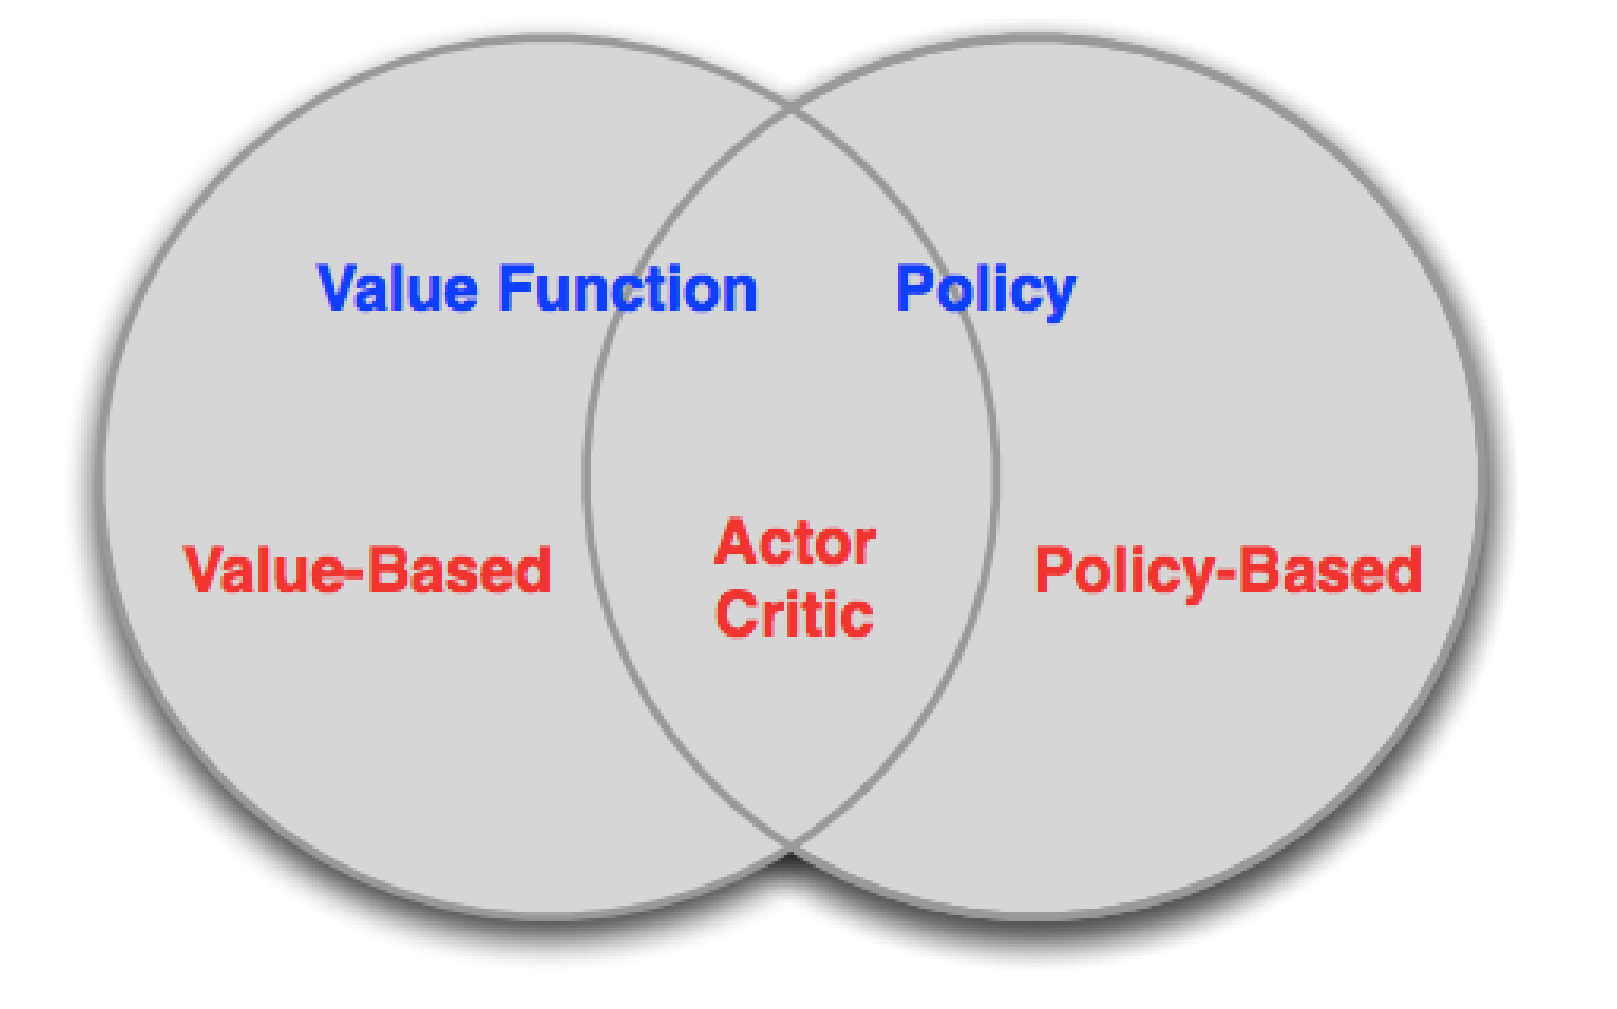
\includegraphics[width=0.7\textwidth,height=0.6\textheight,keepaspectratio]{images/policy-optimization/a2c_2.png}
\end{figure}
\begin{itemize}
    \item \textbf{Value-based} methods (Days 1--2): learn $V$ or $Q$, derive policy implicitly
    \item \textbf{Policy-based} methods (Day 3): learn $\pi_\theta$ directly, no value function
    \item \textbf{Actor-Critic} sits at the intersection: learn \emph{both} a policy \emph{and} a value function
\end{itemize}
\end{frame}
